
\section{Summary}
\label{sec:summary}

In this dissertation I have presented a new probability model for sequence data: the Hierarchical Dirichlet Process Hidden Markov Model with Local Transitions (HDP-HMM-LT, or ``HaMMLeT''), which provides a way to infer a latent state sequence underlying time series data while incorporating prior information that the latent states reside in some similarity space, with transitions being more likely between pairs of states that are nearby in that space.  Two broad versions of the model are presented, which represent similarity fundamentally differently.  

The first version of the model, illustrated in Chapter \ref{chapter:cocktail-party} conceives of similarity as a function of the emission distributions of the respective states; or at least, of a function of the same state information that influences the emission distributions.  This form of the model is well suited to scenarios in which the latent state is a composite of several component sub-states, not all of which change at the same time; that is, the kinds of settings where factorial models are typically used.  The difference between the HaMMLeT model and a facotrial model is that the substates are not modeled as independent sequences in HaMMLeT, and so it is possible to discover correlations among them.  The performance of this model is illustrated in a speaker diarization experiment (the ``cocktail party'' problem), with favorable comparison to both the ``vanilla'' HDP-HMM and the factorial HMM, whose features it combines, as well as to the Sticky HDP-HMM, which privileges self-transitions but possesses no notion of proximity between non-identical states.

The second version of the model, illustrated in Chapter \ref{chapter:music}, represents similarity between states as unrelated to emissions themselves, which is suited to applications where there is a notion of ``functional distance'' between states which is separate from the surface distance between observations at those states, as is arguably the case in Western music, where the ``circle of fifths'' structures harmonic classes in a manner such that consecutive chords tend to be nearby in the circle, even if their pitches are far apart.  This model is illustrated using two harmonic parsing experiments, one using synthetically generated data from the Kulitta grammar \cite{quick2014kulitta}, and the other using Bach chorales.  Comparisons are made to the vanilla HDP-HMM and the Sticky HDP-HMM.  Here, the key finding is that although the two ``non-LT'' models fit the training data well (in fact better than the LT model), they appear to overfit, yielding worse predictive likelihood on a held out test set than the LT model, which evidently recovers a more parsimonious description of the harmonic structure.

I conclude this dissertation by describing some directions for future work extending and further exploring the properties of the HaMMLeT model.  First I describe a potential application related to power disaggregration, which has been a use case for existing nonparametric Bayesian HMMs (e.g., \cite{johnson2013bayesian}).  Then I describe a possible marriage between the local transition property of HaMMLeT with the nonparametric infinite factorial HMM \cite{gael2009infinite}.  Finally, I discuss computational challenges for inference with the HaMMLeT model, and potential directions for improving scalability.


\section{Future Application: Power Disaggregation}
\label{sec:power-disaggregation}

A potential application of the categorical-vector-state model described in Chapter \ref{chapter:cocktail-party} is to disaggregating energy signals.  In the future, I plan to test the model using a subset of the Reference Energy Disaggregation Data set (REDD; \citet{kolter2011redd}).  The data consists of power consumption measurements from several time intervals from several electrical channels in several different homes, as well as an aggregated power consumption time series for each interval per home. An example interval is shown in Fig. \ref{fig:redd-data-example}.  

Two key properties of this data are apparent in the figure.  First, up to some small-scale variability, each channel visits a relatively small number of amplitudes, with some (such as the oven) alternating between an ``on'' state and an ``off'' state, and others (such as the outlets and lighting channels) exhibiting more complex dynamics, presumably corresponding to various appliances or light fixtures turning on and off in different combinations.  This property motivates the choice of a categorical state model.  Second, there are clear correlations among the various channels: in this example, the two oven channels always go on and off together, albeit exhibiting different amplitudes when on, while two of the three lighting channels are highly but not perfectly correlated, while the third exhibits opposing behavior to the other two (perhaps arising from behavior).

Collectively, the dynamics exhibited here are similar to the cocktail party data described in Chapter \ref{chapter:cocktail-party}.  For one, since transitions between combinatorial states tend to be ``local'', in that it is rare for more than one channel to change state at one time, we would expect the HaMMLeT model's bias toward local state transitions to be beneficial, compared to the ``vanilla'' HDP-HMM which has no such locality bias.  On the other hand, not all combinations of states occur in the data, and morever, some state combinations are more or likely than the product of the individual channel probabilities would suggest, suggesting that the flexibility of a model such as HaMMLeT, in which there is a single latent state space over vector-valued states, might be better able to capture the correct transition probaiblities than a model such as the Factorial HMM, in which the component chains evolve {\em a priori} independently.

\begin{figure}[tb]
  \centering
  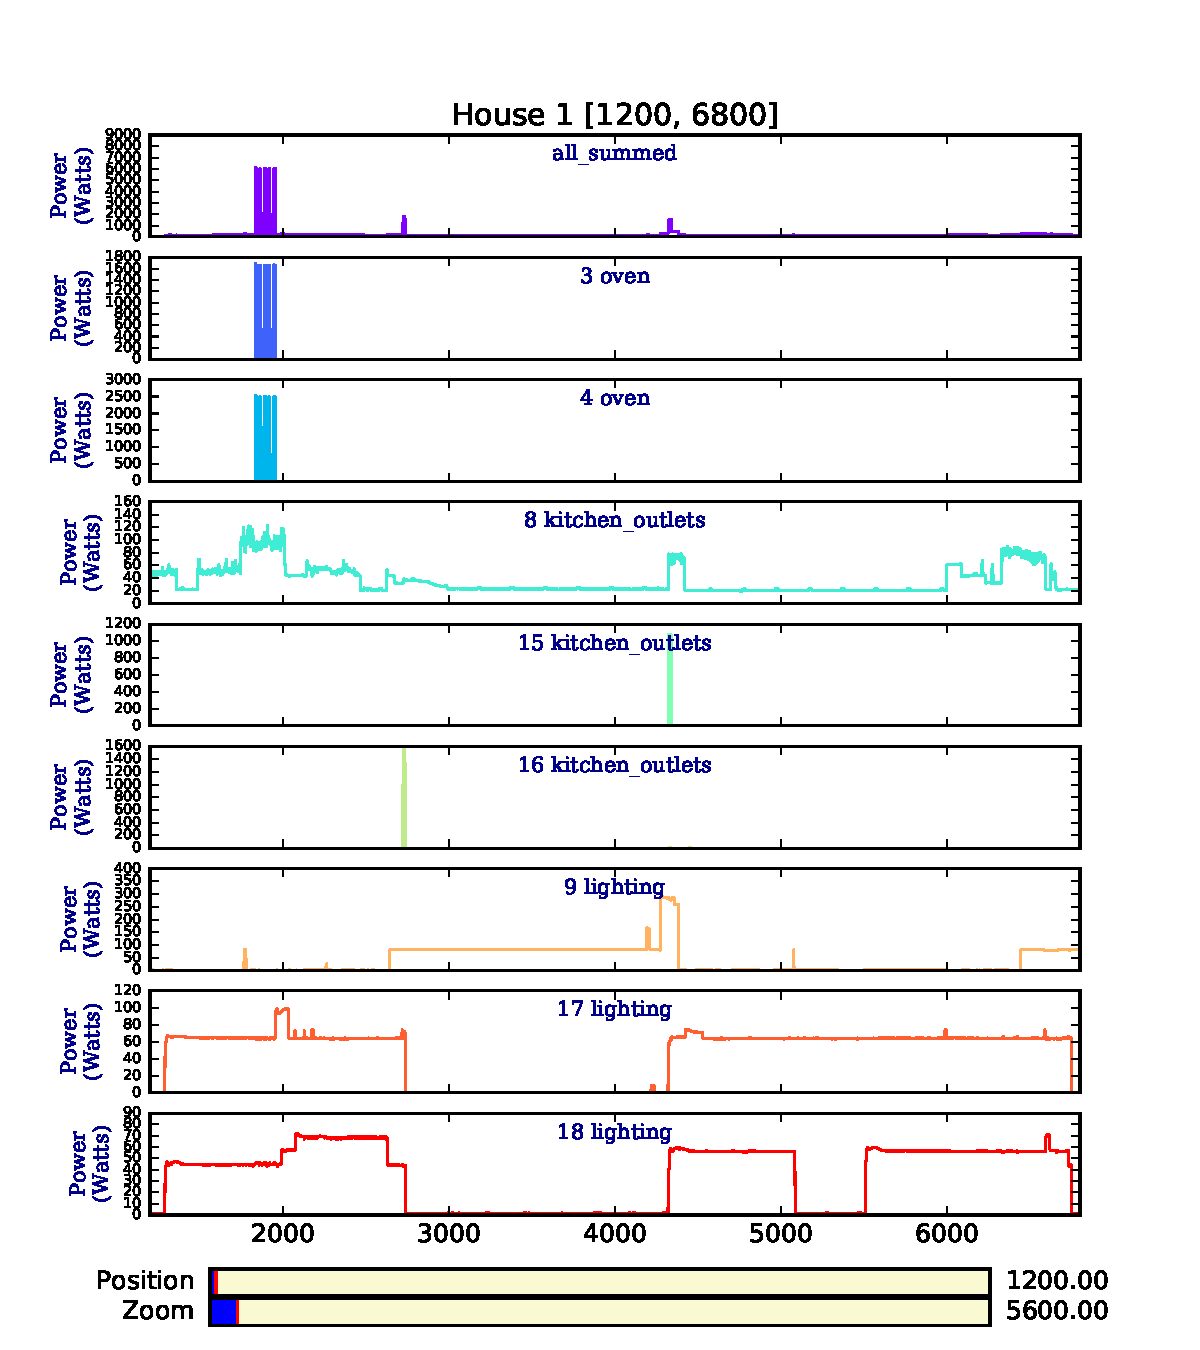
\includegraphics[width=\textwidth]{data/REDD/jw2013_downsampled_intervals/house_1_1200_6800/house_1_1200-6800.pdf}
  \caption{A sample data interval from the REDD dataset \cite{kolter2011redd}.  The top channel contains the total measured power in watts consumed by a home during a period of approximately 24 hours.  Each timestep represents a 20 second intervals, during which the amplitude recorded is a median of the amplitudes in the original higher resolution data.}
  \label{fig:redd-data-example}
\end{figure}

\subsection{Generalizing to Categorical-Valued $\theta$}
It is not difficult to relax the assumption made in Chapter \ref{chapter:cocktail-party} 
that the $\theta_j$ are binary vectors and
instead allow each $\theta_{jd}$ to take on one in an arbitrary set of
discrete values --- i.e., to be categorically distributed rather than
Bernoulli distributed.  The similarity between two states will again be defined in terms of distance between $\theta_j$ vectors that also inform the emission distribution via a linear-Gaussian model.  As a result, much of the additional inference steps described for the 
cocktail party experiment carry over to this instantiation of the
model.  The exception of course is
inferences about $\theta$.

In this section, I define representations and priors for $\theta$ and the weight matrix, 
$W$ for the general case of categorical-vector-valued $\theta$.  Then
I derive the necessary Gibbs steps.  

A potential future application of this version of the model to power
disaggregation is described in Chapter \ref{chapter:discussion}, where the observations consist of an aggregated energy-use time series from several houses, the latent state vector describes the energy being used by each of several channels (e.g., lighting, refrigerator, washer/dryer), such that individual channels are in one of several discrete states at a given time. For example, the refrigerator channel might cycle between an ``off'' state, a low-power standby state, and a high-power ``active cooling'' state.  Inference consists of discovering the set of discrete states for each channel, attributing a typical level of energy consumption for each state, and inferring what state each channel is in during each discretized time window in the data.

\subsection{Priors and Representations in the Categorical State Variant}
\label{sec:priors-repr-categ}

In place of Beta priors on each $\theta_{jd}$, we can use Chinese
Restaurant Process priors, with concentration parameter
$\alpha_{d}^{(\theta)}$.  In the case that the number of categorical 
values is known in advance, this can be replaced by a Dirichlet 
prior, but I present the more flexible case here. 

The weight matrix $W$ must be expanded to allow for distinct weights
associated with each possible value of the $\theta_{jd}$.  Rather than
the matrix given by $(w_{dk})_{d=1,\dots,D,k=1,\dots,K}$, we now need
a set of weights, $(w_{sdk})$, where $s$ indexes the categorical
values that $\theta_{jd}$ can take.  With a CRP prior, 
there is an unbounded number of $s$, though during inference, as in the direct assignment sampler for the HDP-HMM, we need only consider those values to which some state is currently assigned, plus one additional value representing a ``new'' state.

I will continue to assume that the $\phi$ function
decays exponentially as a function of the number of component-wise
differences (that is, Hamming distance) 
between a pair of states.  Specifically, $\Delta_{jj'd}$ is zero
if and only if $\theta_{jd} = \theta_{j'd}$ and is 1 otherwise,
$\Delta_{jj'} = \sum_{d} \Delta_{jj'd}$, and
$\phi(\theta_{j}\theta_{jj'}) = e^{-\lambda\Delta_{jj'}}$.
  
We can use a ``dummy variable'' representation
of $\theta_j$.  Define $S_d$ to be the number of realized
states for dimension $d$ and a 1 in position $\sum_{d' < d} S_{d'} + s$ indicates that
$\theta_{jd} = s$.  There will thus be $D$ entries equal to 1, with
the remaining entries equal to zero.  We can then represent the weight
matrix $\bW$ as stacked block matrix, where each block is $S_d
\times K$, and there is one block for each $d$.  In practice we only
need to instantiate a new block when some $\theta_{jd}$ is assigned to
a ``new table'' in the CRP metaphor, so that the dimension of $\bW$ is
$\sum_d S_d \times K$.  Then we have
\begin{equation}
  y_{t} \sim \Norm{w^{(b)} + W^{\sf T}\theta_{z_t}}{\Sigma}
\end{equation}
where $w^{(b)}$ is a $K$-dimensional bias vector with a separate Normal
prior, $W$ is the weight matrix as defined just above, $z_t$ is the
state indicator for time $t$, and $\Sigma$ is a $K \times K$ noise covariance matrix.

\subsection{Adapting Posterior Inference for Categorical State Vectors}
\label{sec:adapt-post-infer}

\paragraph{Sampling $\theta$}

As before, the conditional posterior for $\theta_{jd}$ 
is proportional to the product of three terms: the prior (now a CRP),
the likelihood of all successful and failed transitions to and from
state $j$, and the likelihood of the observation sequence.

Under the CRP, the probability that $\theta_{jd} = s$ conditioned on the rest of $\theta$ (but not the data) is proportional to the number of other $j' \neq j$ such that
$\theta_{j'd} = s$ where this count is positive; and proportional to
$\alpha_j^{(\theta)}$ otherwise.  Let 
\begin{equation}
\tilde{n}^{-j}_{ds} = \sum_{j' \neq j} I(\theta_{jd} = s), \quad s = 1,
\dots, S_d
\end{equation}
be these counts, where we assume that there are $S_d$ distinct values
taken by the $\theta_{jd}$ for a particular $d$.  Then
\begin{equation}
  p(\theta_{jd} = s \given \theta_{d}^{-j}) \propto
\begin{cases}
\tilde{n}^{-j}_{ds} & s = 1, \dots, S_d \\
\alpha_{d}^{(\theta)} & s = S_d + 1
\end{cases}
\end{equation}

The transition component of the likelihood is as in the binary case:
\begin{align}
  p(z, Q \given \theta_{jd}, \theta_{d}^{-j}) & \propto
  e^{-\lambda\sum_{j'} \Delta_{jj'} (n_{jj'} + n_{j'j})} \prod_{j'
    \neq j} (1 - e^{-\lambda\Delta_{jj'} (q_{jj'} + q_{j'j})})\\
  &\propto e^{-\lambda \sum_{j'} I(\theta_{jd} \neq \theta_{j'd})
    (n_{jj'} + n_{j'j})} \prod_{j'
    \neq j} (1 - a\cdot e^{-\lambda I(\theta_{jd} \neq \theta_{j'd}) (q_{jj'} + q_{j'j})})
\end{align}
where $a$ is a constant in $\theta_{jd}$, defined as $e^{-\lambda
  \Delta_{jj'-d} (q_{jj'd} + q_{j'jd})}$.  Taking a log yields
\begin{equation}
  \log p(z, Q \given \theta_{jd}, \theta_{d}^{-j}) =
  -\lambda \sum_{\{j':\ \theta_{jd} \neq \theta_{j'd}\}} (n_{jj'} +
  n_{j'j}) + \sum_{j'
    \neq j} \log(1 - a\cdot e^{-\lambda I(\theta_{jd} \neq \theta_{j'd}) (q_{jj'} + q_{j'j})})
\end{equation}

The emission component of the likelihood is given for each $t$ by
\begin{equation}
  p(y_t \given \theta_{z_t}, W, \Sigma) \propto \abs{\Sigma}^{-1/2}
  \exp(-\frac{1}{2} (y_t - w^{(b)} -
  W^{\sf T} \theta_{z_t})^{\sf T}\bSigma^{-1}(y_t - w^{(b)} - W^{\sf T} \theta_{z_t}))
\end{equation}

Assuming a diagonal covariance matrix, isolating $\theta_{j,d}$, and
taking a log, this becomes, for each $k$ and $t$,
\begin{align}
  \log p(y_{tk} \given \theta_{z_t,d}, \theta_{z_t}^{-d}, w^{(b)}_k, \sigma^2_k) &=
   -\frac{1}{2\sigma^2_k} \left(y_{tk} -
      w^{(b)}_k-\theta_{z_t}\bw_k\right)^2 \\
  &\propto -\frac{1}{2\sigma^2_k} (\sum_{d'} w_{\theta_{z_td'},d',k} -
    (y_{tk} - w^{(b)}_k))^2 \\
  &\propto -\frac{1}{2\sigma^2_k}(w_{\theta_{z_td},d,k} - (y_{tk} -
    w^{(b)}_k - \sum_{d' \neq d} w_{\theta_{z_t,d'},d',k}))^2
\end{align}
For a particular $j$ and $d$, the full emission log likelihood is a sum of
terms like the above, over all $t$ such that $z_t = j$.

\paragraph{Sampling $W$}
Having expanded $\theta$ to a dummy variable representation, and
having constructed a stacked block form of $W$, we can sample each
column of $W$ from a conditional posterior multivariate Normal just
as in the binary case.

\paragraph{Sampling $\lambda$} Since $\lambda$ controls only the relationship between the distance matrix, $\Delta$, and the similarity matrix, $\phi$, upon 
conditioning on $\Delta$ and the jump attempts, $\lambda$ is not sensitive to the way that $\Delta$ was computed; hence it can be sampled using Adaptive Rejection Sampling from exactly the same conditional distribution as before.

\section{Scaling Inference Using Beam Sampling}
\label{sec:scal-infer-using}

A limitation of the weak limit approximation defined in this dissertation and 
used to carry out Gibbs sampling in all experiments discussed is that requires a maximum number of states (referred to as $J$ in the text) to be specified in advance.  
Although $J$ can be set as large as desired to approximate a truly infinite 
state model, and the hierarchical structure of the HDP prior ensures that a 
sparse subset of available states will be used, the inference algorithm scales 
quadratically in $J$ (specifically, on the order of $\mathcal{O}(TJ^2)$, where 
$T$ is the number of observations), due to the multiplication by the transition matrix that must occur during the forward message passing step.  Hence it may be quite costly to 
perform inference if a very large $J$ is needed.  Because of this, inference algorithms that scale better and, ideally, eliminate entirely 
the need for the upper bound on the size of the state space.

A promising possibility comes from {\bf beam sampling} \cite{vangael2008beam}, which 
in the ordinary HDP-HMM allows the $z_t$ to be sampled jointly
from the full infinite state HDP model without evaluating all state combinations at every $t$.
This is achieved through {\bf slice sampling} \cite{neal2003slice}.  Slice sampling is a Gibbs
sampling method in which the goal of sampling values $x$ from a target
density, $f(x)$ is achieved by the introduction of an auxiliary
``slice'' variable, $s$ that depends on $x$ according to the density 
$f(s \given x)$, chosen so that $f(x \given s)$ can be sampled from
easily.  By the usual logic of a Gibbs sampler, in the limit we obtain
samples from the joint distribution $f(x,s)$, the $x$-marginal of
which is $f(x)$.

\subsection{Beam Sampling in the Original HDP-HMM}
\label{sec:beam-sampl-orig}

Beam sampling \citep{vangael2008beam} combines slice sampling with the
forward-backward algorithm as follows.  The original conditional
distribution of each $z_t$ is given by the transition matrix:
\begin{align}
  p(z_t = j' \given z_{t-1} = j, \pi) = \pi_{jj'}
\end{align}
For each $t$ we introduce a slice variable, $s_t$, which is uniformly
distributed on the interval $(0, \pi_{z_{t-1}z_t})$, so that we have
the conditional density
\begin{align}
  p(s_t \given z, \pi) = \pi_{z_{t-1}z_t}^{-1} \mathbb{I}(0 < s_t < \pi_{z_{t-1}z_t})
\end{align}
This yields the joint density
\begin{align}
  p(z, s \given \pi) &= \prod_{t=1}^T \pi_{z_{t-1}z_t}
  \pi_{z_{t-1}z_t}^{-1} \mathbb{I}(0 < s_t < \pi_{z_{t-1}z_t})\\
  &= \prod_{t=1}^T \mathbb{I}(0 < s_t < \pi_{z_{t-1}z_t}),
\end{align}
that is, conditioned on the collection of slice variables (but not yet
conditioned on the data), the distribution of state sequences is
uniform over all sequences that meet the condition that
$\pi_{z_{t-1}z_t} > s_t$ for all $t$.

Since for each $j$, the transition probabilities, $\pi_{jj'}$ must sum
to 1 over all $j'$, there can be only a finite number of choices for
$j'$ at each $t$ that satisfy $\pi_{jj'} > s_t$; hence, conditional on
$s$, we need only consider finitely many states during the forward and
backward steps.

Now, conditioning on the data $y$ as well, and defining
$b^*_{t+1}(j') := p(z_{t+1} = j' \given s, y_1, \dots, y_{t+1})$, 
the forward message passing recurrence relation becomes
\begin{align}
  b^*_{t+1}(j') &= p(z_{t+1} = j' \given s, y_1, \dots, y_{t+1})\\
  &\propto p(z_{t+1} = j', s, y_1, \dots, y_{t}) p(y_{t+1} \given z_{t+1} = j') \\
  &= p(y_{t+1} \given z_{t+1} = j') \sum_{j} p(z_{t} = j, z_{t+1} = j', s, y_1, \dots, y_{t}) \\
  &= p(y_{t+1} \given z_{t+1} = j') \sum_{j} p(z_{t} = j, s, y_1, \dots, y_{t})
  p(z_{t+1}  = j' \given z_{t} = j, s) \\
  &\propto f(y_{t+1} \given \theta_{j'}) \sum_{j} b^*_{t}(j) I(\pi_{jj'} > s_{t+1}) 
\end{align}
Although the sum over $j$ is still technically over an infinite number
of terms, we can show that only finitely many $j$ will have
$b^*_{t}(j) > 0$.

First, consider $b^*_1$.  We have
\begin{align}
  b^*_1(j') &\propto f(y_{1} \given \theta_{j'}) I(\pi_{0j'} > s_t) .
\end{align}
Since only finitely many entries in the initial distribution $\pi_0$
can exceed $s_t$, $b^*_1(j')$ is 0 for all but finitely many $j'$.
Now suppose that $b^*_t(j)$ is positive for finitely many $j$.  Denote
this set by $\mathcal{J}_t$.  In order for $b^*_{t+1}(j')$ to be
positive, we need to have $\pi_{jj'} > s_{t+1}$ for some $j \in
\mathcal{J}_t$.  Since for each $j$, there are finitely many $j'$ satisfying
$\pi_{jj'} > s_{t+1}$, and since there are finitely many $j \in
\mathcal{J}_t$, there can be only finitely many $\pi_{jj'} > s_{t+1}$ across
{\em all} combinations of $j$ and $j'$.  Hence, $b^*_{t+1}$ has finite support.

The backward distribution for sampling $z_{t}$ given $z_{t+1}$ and $y$
data becomes
\begin{align}
  p(z_t = j \given z_{t+1}, s, y) &\propto p(z_{t} = j \given s, y_1,
  \dots, y_{t}) p(z_{t+1} \given z_t, s) \\
  &= b^*_{t}(j) I(s_{t+1} > \pi_{jz_{t+1}})
\end{align}
which is again zero for all but finitely many $j$.

Using this algorithm we can represent only those entries in the
transition matrix $\pi$ that are needed, combining the mass of all
unrepresented components into one value, $\pi_{j,new}$ for each
$j$.  When performing the forward step, each time there is a $t$ and
$j$ such that both $b^*_{t}(j) > 0$,$\pi_{j,new} > s_{t+1}$, then it is possible that the chain could visit a
new state, and so we perform a stick-breaking step to instantiate the
new component, and the new transition probabilities to and from that
component.  Let $J$ be the number of states currently instantiated, so
that the current representation of $\beta$ is $\beta_1, \dots,
\beta_J, \beta_{new}$.  Then, to instantiate a new component, sample
\begin{align}
  \tilde{\beta}_{J+1} \sim \Beta{1}{\gamma}
\end{align}
set
\begin{align}
  \beta_{J+1} \gets \tilde{\beta}_{J+1} \beta_{new} \qquad \beta_{new}
  \gets (1 - \tilde{\beta}_{J+1}) \beta_{new}
\end{align}
and for each $j = 1, \dots J$, sample
\begin{align}
  \tilde{\pi}_{j,J+1} \sim \Beta{\alpha \beta_{J+1}}{\alpha \beta_{new}}
\end{align}
and set
\begin{align}
  \pi_{j,J+1} \gets \tilde{\pi}_{j,J+1} \pi_{j,new} \qquad \pi_{J,new}
  \gets (1 - \tilde{\pi}_{j,J+1}) \pi_{j,new}
\end{align}
Now, if $\pi_{j,J+1} > s_{t+1}$ for some $j$ in the support of
$b^*_t$, then $J+1$ will be in the support of $b^*_{t+1}$, and we need
to sample a new transition distribution from state $J+1$ according to
\begin{align}
  (\pi_{J+1,1}, \dots, \pi_{J+1,J+1}, \pi_{J+1,new}) \sim \Dir{\alpha
    \beta_1, \dots, \alpha \beta_{J+1}, \alpha \beta_{new}}.
\end{align}
The above process is repeated until $\pi_{j,new} < s_{t+1}$ for all $j$,
after which we can calculate $b^*_{t+1}$ and then move on to the next $t$.

\subsection{Adapting Beam Sampling to the HDP-HMM-LT}
\label{sec:adapt-beam-sampl}

In the context of the weak limit approximation to the HDP-HMM-LT, we compute the entire transition matrix, with entries proportional to $\pi_{jj'}\phi_{jj'}$.  When the number of states is bounded above by $J$, the beam sampling algorithm described above can be used directly, except that all $J^2$ transition probabilities are represented explicitly, and so there is no need for the $\pi_{new}$ term and the corresponding stick-breaking step.  Using beam sampling in this manner can greatly speed up the process of sampling the $z_t$, and thus although it does not remove the need to specify $J$, it allows larger $J$ to be used without the quadratic scaling in computational complexity.

Ideally we would like to remove entirely the need to specify $J$.  Unfortunately in the HDP-HMM-LT, the aggregated probability of transitioning to some new state is
\begin{align}
  \sum_{j'=J+1}^{\infty} \pi_{jj'}\phi_{jj'}
\end{align}
which cannot in general be sampled directly, since unlike in the special case when all $\phi_{jj'}$ are identical, the prior on this quantity is not a Gamma distribution.  A related issue for the Markov Jump Process with Failed Transitions (MJP-FT) representation is that the auxiliary variables $\tilde{u}_t$, representing the continuous duration of interval between transitions $t$ and $t+1$ have distributions defined in terms of the sum of transition probabilities:
\begin{align}
  \tilde{u}_t \given z_t, \pi, \phi &\sim \Exp{\sum_{j'=1}^\infty \pi_{z_t,j'}\phi_{z_t,j'}}
\end{align}

It may be possible to get around this issue through the introduction of additional or modified slice variables.  This is an interesting direction for future work.

\section{An Infinite Factorial HDP-HMM-LT}
\label{sec:an-infin-fact}

One setting in which a local transition property is
desireable is the case where the latent states indicate which in a set
of hidden features is ``active'' at time $t$; that is, when the latent
state is represented by a binary vector.  A parametric example of such
a model is the Factorial HMM \cite{ghahramani1997factorial},
nonparametric extensions of which, such as the infinite factorial
hidden Markov Model \cite{gael2009infinite} and the infinite factorial dynamic model
\cite{valera2015infinite}, have been developed in recent years
by making use of the Indian Buffet Process
\cite{ghahramani2005infinite} as a state prior.  It would be
conceptually straightforward to combine the IBP state prior with the
similarity bias of the LT model, provided the chosen similarity
function is uniformly bounded above on the space of infinite length
binary vectors (for example, take $\phi(u,v)$ to be the exponentiated
negative Hamming distance between $u$ and $v$).  Since the number of
differences between two draws from the IBP is finite with probability
1, this yields a reasonable similarity metric.

Implementing and exploring this variant of the model is another direction of future research.
